%% manuscript_anonymous.tex — Technovation (Elsevier, Q1, IF=10.9)
%% Anonymized version for double-blind review
%%
%% Compile: pdflatex manuscript_anonymous.tex → bibtex manuscript_anonymous → pdflatex (×2)
%% -----------------------------------------------------------------

\documentclass[5p,times,authoryear]{elsarticle}

%% ----- Packages -------------------------------------------------
\usepackage{amsmath,amssymb}
\usepackage{graphicx}
\usepackage{booktabs}
\usepackage{hyperref}
\usepackage{natbib}
%\usepackage{lineno}          % line numbering for review
\usepackage{xcolor}
\usepackage{float}
\usepackage{multirow}
\usepackage{subcaption}
\usepackage[utf8]{inputenc}
\usepackage[T1]{fontenc}
\usepackage{threeparttable}
\usepackage{placeins}        % \FloatBarrier
\usepackage{tabularx}
\usepackage{array}
\usepackage{bbm}             % \mathbbm{1} for indicator functions
%\usepackage{orcidlink}       % ORCID icons (removed for anonymous review)
\usepackage{adjustbox}       % auto-fit wide tables

%% ----- Line numbering (required for review) ---------------------
%\modulolinenumbers[5]

%% ----- Journal metadata -----------------------------------------
\journal{Technovation}

%% =================================================================
%%  HIGHLIGHTS (Elsevier required element)
%% =================================================================
\begin{highlights}
\item Minimum wage shocks reduce automation investment 16.7\% in Colombian manufacturers
\item Cash-constrained firms absorb cost shocks rather than automating: a dual economy trap
\item Informality acts as an escape valve, absorbing labor displaced by wage increases
\item Automation potential and formality, not labor cost, drive sectoral vulnerability
\item Standard OECD automation models mispredict technology adoption in dual economies
\end{highlights}

%% =================================================================
%%  FRONTMATTER
%% =================================================================
\begin{document}

\begin{frontmatter}

%% ----- Title ----------------------------------------------------
\title{Technology Adoption in Dual Economies: How Informality and Non-Wage Labor Costs Shape Automation Dynamics --- Evidence from Colombia}

%% ----- Authors (removed for double-blind review) -----------------
%% Author names, emails, ORCIDs, and affiliations are provided
%% in the separate title page document.

%% ----- Abstract -------------------------------------------------
\begin{abstract}
Standard automation theory predicts that rising labor costs accelerate technology adoption. We test this in Colombia---a dual economy where 55.8\% of employment is informal and non-wage costs add 46--58\% to base wages---using a difference-in-differences design exploiting minimum wage shocks under the Petro administration (+16\% in 2023, +12\% in 2024). Contrary to theory, firms most exposed to these shocks \emph{reduced} automation investment per worker by 16.7\% ($p=0.045$). This counterintuitive result reflects the ``dual economy trap'': in cash-constrained economies with large informal sectors, wage increases consume firm margins rather than redirecting capital toward labor-replacing technologies, while informality provides an escape valve absorbing displaced formal labor. Using 66,775 firm-year observations from the Annual Manufacturing Survey and 364,998 individual observations from household labor force data, we find null effects on sectoral formality rates and automation risk composition. Principal component analysis of our sectoral vulnerability index confirms that automation potential and formality---not labor cost alone---drive vulnerability rankings. These findings challenge the universality of the cost--automation nexus and carry implications for minimum wage policy, parafiscal reform, and technology subsidies in economies where informality exceeds 30\% of employment.
\end{abstract}

%% ----- Graphical abstract placeholder ---------------------------
%%\begin{graphicalabstract}
%%  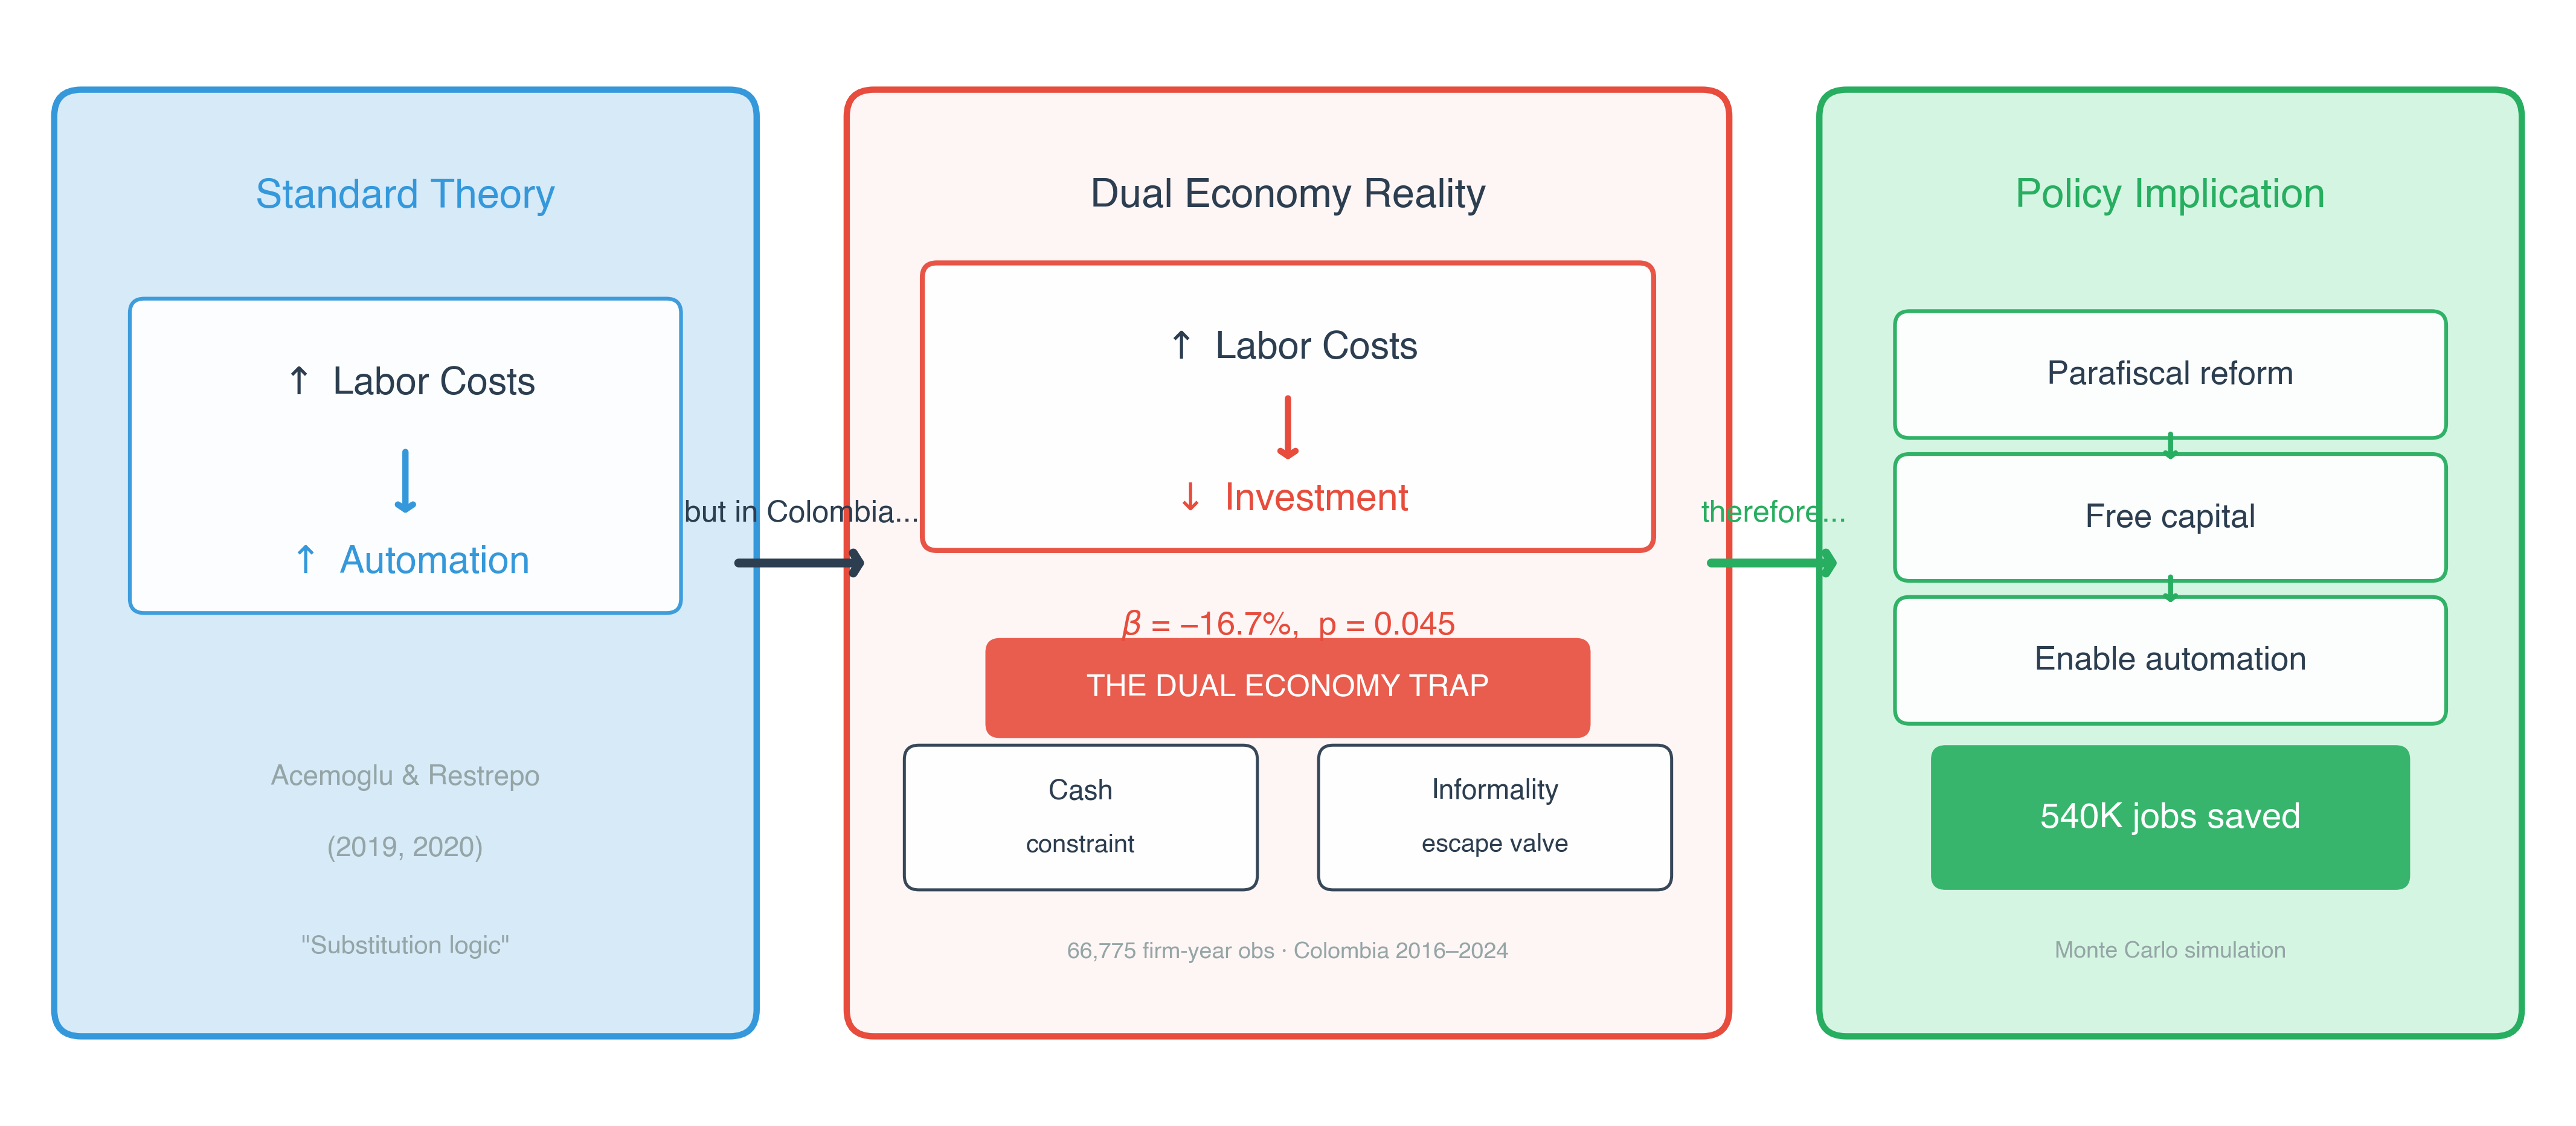
\includegraphics[width=\textwidth]{graphical_abstract.pdf}
%%\end{graphicalabstract}

%% ----- Keywords -------------------------------------------------
\begin{keyword}
  Automation \sep Labor costs \sep Dual economy \sep Informality \sep
  Minimum wage \sep Difference-in-differences \sep Colombia
\end{keyword}

\end{frontmatter}

%% ----- Line numbers start here ----------------------------------
%\linenumbers

%% =================================================================
%%  1. INTRODUCTION
%% =================================================================
\section{Introduction}
\label{sec:introduction}

Since \citet{frey2017future} estimated that 47\% of US employment faces high automation risk, a growing literature has quantified these risks across countries and occupations \citep{arntz2016, webb2020, eloundou2023gpts}. Yet this research overwhelmingly focuses on advanced economies with universal formal employment and developed capital markets. The roughly 2 billion workers in developing countries---where informality often exceeds 50\% and firms face severe capital constraints---remain outside the analytical frame \citep{laporta2014, arias2023informality}.

The task-based framework of \citet{acemoglu2019automation} and its extensions \citep{acemoglu2020robots, acemoglu2022tasks} predict that rising labor costs accelerate technology adoption, a mechanism supported empirically in the US \citep{acemoglu2020robots}, Germany \citep{dauth2021}, Japan \citep{adachi2022}, and Spain \citep{koch2021}. The implicit assumption is that firms have access to capital, operate within formal regulatory frameworks, and substitute capital for labor along a smooth production frontier.

Colombia presents a stark test. With robot density of 2--5 per 10,000 manufacturing workers versus 1,012 in South Korea \citep{ifr2024}, the country invests roughly one-tenth of what its labor costs would predict internationally. This ``automation gap'' persists despite non-wage costs adding 46--58\% to base wages \citep{anif2018}, while 55.8\% of workers operate informally \citep{arias2023informality}. This combination creates what we term a \emph{dual economy trap}: an institutional configuration in which labor cost shocks fail to generate the predicted automation response.

We exploit a natural experiment to test this hypothesis directly. Between 2023 and 2024, Colombia's minimum wage increased by 16\% and 12\% in nominal terms, respectively, under the administration of President Gustavo Petro---far exceeding productivity growth of 1--2\% per year. These shocks affected firms differentially based on their pre-existing labor cost structure. Using a difference-in-differences (DiD) design with continuous treatment intensity measured by pre-treatment (2022) labor cost share of gross production, we estimate the causal effect of these cost shocks on firm-level automation investment.

Our central finding is counterintuitive: firms most exposed to minimum wage increases \emph{reduced} investment per worker by 16.7\% relative to less exposed firms ($\beta = -0.167$, $p = 0.045$), and their investment rates declined by 0.7 percentage points ($p = 0.009$). Rather than accelerating technology adoption, large labor cost shocks in a cash-constrained, dual economy appear to freeze capital investment. We interpret this through three mechanisms: (i) a \emph{cash constraint} channel, whereby wage increases consume the operating margins that would otherwise finance automation capital; (ii) an \emph{informality escape valve}, whereby firms shift labor arrangements toward informal contracts rather than investing in technology; and (iii) an \emph{uncertainty freeze}, whereby regulatory volatility under rapid minimum wage increases discourages long-term capital commitments.

Complementing the firm-level analysis, we examine 364,998 individual-level observations from Colombia's GEIH household survey (2022--2024), finding null effects on both formality rates ($\beta = +0.002$, $p = 0.688$) and the automation risk composition of employment ($\beta = -0.004$, $p = 0.132$). PCA validation of our sectoral vulnerability index confirms that automation potential (loading = 0.44) and formality (0.42) dominate, while labor cost receives only 0.14 weight---corroborating that in dual economies, task content and institutional formality, not cost alone, determine automation vulnerability.

This paper makes three contributions. First, it provides the first quasi-experimental evidence on the causal effect of labor cost shocks on automation investment in a developing country with a large informal sector, exploiting exogenous variation that no prior study has identified in this setting \citep{graetz2018, koch2021, bid2023, morales2023risk}. Second, we articulate the ``dual economy trap'' as a theoretical mechanism explaining why cash constraints, informality, and regulatory uncertainty cause labor cost increases to \emph{reduce} rather than redirect investment. Third, PCA validation demonstrates that sectoral automation vulnerability is driven by task-level automation potential and formality rather than labor cost---with direct implications for policy prioritization.

The remainder of the paper proceeds as follows. Section~\ref{sec:theory} develops the theoretical framework, extending the task-based model to dual economies and deriving testable predictions. Section~\ref{sec:context} describes the institutional context of Colombian labor costs and informality. Section~\ref{sec:data} presents the data sources, identification strategy, and econometric specifications. Section~\ref{sec:results} reports the main results, event studies, and robustness checks. Section~\ref{sec:policy} discusses theoretical and policy implications and the generalizability of our findings to other developing economies. Section~\ref{sec:limitations} addresses limitations and future research directions. Section~\ref{sec:conclusion} concludes.

\FloatBarrier


%% =================================================================
%%  2. THEORETICAL FRAMEWORK
%% =================================================================
\section{Theoretical Framework: Automation in Dual Economies}
\label{sec:theory}

\subsection{The Task-Based Framework}
\label{subsec:task_model}

We build on the task-based model of \citet{acemoglu2019automation}, which provides a unified framework for analyzing how automation reshapes labor markets through three channels: displacement, reinstatement, and productivity effects. In this framework, production requires the completion of a continuum of tasks $i \in [0,1]$, each of which can be performed by labor or capital. At any point in time, there exists a threshold task $I^*$ such that all tasks $i < I^*$ are automated and all tasks $i \geq I^*$ are performed by labor. Technology adoption shifts this threshold to the right, displacing workers from tasks that machines can now perform more cheaply.

The firm's automation decision depends on the relative cost of labor versus capital for each task. For a representative task $i$, the firm automates when:
\begin{equation}
\label{eq:automation_threshold}
\frac{w + c}{r \cdot \alpha(i)} > 1
\end{equation}
where $w$ is the base wage, $c$ represents non-wage labor costs (social contributions, severance, parafiscal charges), $r$ is the user cost of capital, and $\alpha(i)$ captures the productivity of machines at task $i$. In the standard model, an increase in total labor costs $(w + c)$ unambiguously shifts the automation threshold to the right: more tasks become cheaper to automate, and the displacement effect dominates in the short run.

\citet{acemoglu2022tasks} show that automation need not reduce aggregate labor demand if productivity gains create new labor-intensive tasks, but this balance depends on technology quality. \citet{acemoglu2020taxes} introduce ``so-so technologies''---automation that displaces labor without large productivity gains---showing that excessive adoption of mediocre technologies can reduce welfare.

\subsection{Extension to Dual Economies: The Formality Paradox}
\label{subsec:dual_economy}

The standard framework assumes that all labor operates within a unified formal market: workers receive regulated wages, firms pay mandated contributions, and automation decisions reflect the full cost of formal employment. In dual economies, this assumption is violated. Following \citet{laporta2014} and \citet{ulyssea2018}, we model the labor market as comprising two segments---a formal sector with regulated wages and non-wage costs, and an informal sector with flexible compensation and minimal regulatory burden.

Let $\lambda \in [0,1]$ denote the economy's formality rate. The effective labor cost faced by a representative firm depends on its workforce composition:
\begin{equation}
\label{eq:effective_cost}
\tilde{w} = \lambda(w + c) + (1-\lambda) w_I
\end{equation}
where $w_I < w$ is the informal wage. This creates what we term the \emph{formality paradox}: formal workers generate the non-wage costs that theoretically incentivize automation, but only formal-sector firms have the organizational capacity, capital access, and regulatory incentives to adopt labor-replacing technologies. Informal firms, which account for the majority of employment in countries like Colombia, Brazil, and India, neither generate the cost pressure nor possess the means to automate.

This paradox implies that (i) aggregate automation responses are attenuated by the informal employment share, (ii) informality provides an ``escape valve'' allowing firms to shift workers to informal arrangements rather than investing in technology, and (iii) equilibrium automation depends not only on the labor--capital cost differential but also on the formal--informal labor cost differential.

\subsection{Cost-Induced versus Efficiency-Induced Adoption}
\label{subsec:cost_vs_efficiency}

The distinction between cost-induced and efficiency-induced technology adoption is central to understanding automation dynamics in developing countries. Cost-induced adoption occurs when rising labor costs push firms past the automation threshold in Equation~\ref{eq:automation_threshold}---the standard mechanism emphasized by \citet{acemoglu2019automation} and supported empirically by \citet{koch2021} and \citet{adachi2022}. Efficiency-induced adoption occurs when improvements in automation technology (increases in $\alpha(i)$) make capital more productive at performing specific tasks, regardless of labor costs.

In advanced economies, both channels operate simultaneously: high wages incentivize cost-induced adoption, while proximity to technological frontiers facilitates efficiency-induced adoption. In developing economies, cost-induced adoption may be the primary channel because firms are further from the technological frontier and rely on imported, standardized automation technologies. However, this channel requires that firms have sufficient liquidity and capital access to respond to cost signals---a condition that is far from guaranteed in economies with underdeveloped financial markets and high credit constraints \citep{busso2020}.

The nature of the technologies available to developing-country firms also matters. Much of the automation capital accessible to Colombian manufacturers falls into the ``so-so'' category identified by \citet{acemoglu2020taxes}: basic industrial robots and process automation that displace routine tasks without generating transformative productivity gains. This makes the investment decision more marginal and more sensitive to cash flow constraints.

\subsection{The Dual Economy Trap: A Formal Characterization}
\label{subsec:formal_trap}

We now formalize the intuition that labor cost shocks can inhibit rather than promote automation in cash-constrained economies. Consider a representative formal-sector firm that chooses between labor $L$ and automation capital $K_A$ to produce output $Y = F(K_A, L)$. The total cost of a formal worker is $w(1 + \tau)$, where $w$ is the base wage and $\tau \in [0.46, 0.58]$ is the non-wage surcharge comprising social security, mandatory provisions, and parafiscal charges as documented in Section~\ref{subsec:labor_costs}. Let $r_A$ denote the rental (user) cost of automation capital.

In each period, the firm earns operating profits:
\begin{equation}
\label{eq:profits}
\pi = pY - w(1+\tau)L - r_A K_A - F_C
\end{equation}
where $p$ is the output price and $F_C$ represents fixed costs. The standard cost--automation prediction follows directly: the firm invests in an additional unit of automation if the marginal product of automation capital exceeds its rental cost, i.e., $\partial F / \partial K_A > r_A / p$. An increase in $w(1+\tau)$ raises the relative cost of labor and, assuming some substitutability, makes the automation margin more attractive.

However, this reasoning assumes that the firm can finance the required upfront investment. Automation capital is lumpy: adopting a new technology requires an indivisible expenditure $C_A$ (e.g., purchasing an industrial robot, installing process automation software, or restructuring production lines). In developing economies with thin capital markets and high collateral requirements, this expenditure must typically be financed from retained earnings \citep{busso2020}. The firm can invest in automation only if:
\begin{equation}
\label{eq:finance_constraint}
\pi \geq C_A
\end{equation}

Now consider a minimum wage shock $\Delta w > 0$. This shock has two simultaneous effects. First, it increases the total labor cost $w(1+\tau)$, which raises the return to automation and should incentivize investment---the standard channel. Second, it reduces operating profits:
\begin{equation}
\label{eq:profit_reduction}
\Delta \pi = -(1+\tau) L \cdot \Delta w < 0
\end{equation}

The dual economy trap emerges when the profit reduction is large enough to push the firm below the financing threshold. Formally, a firm is ``trapped'' when:
\begin{equation}
\label{eq:trap_condition}
\pi_0 \geq C_A \quad \text{but} \quad \pi_0 - (1+\tau)L \cdot \Delta w < C_A
\end{equation}
where $\pi_0$ denotes pre-shock profits. The trap condition is more likely to bind when: (i) the non-wage surcharge $\tau$ is large (amplifying the cost shock), (ii) the firm is labor-intensive (large $L$ relative to revenue), (iii) initial margins are thin ($\pi_0$ is close to $C_A$), and (iv) the wage shock $\Delta w$ is large. All four conditions characterize the Colombian manufacturing sector.

In advanced economies, condition~\eqref{eq:finance_constraint} typically does not bind because firms can access external capital markets---bank credit, bond issuance, or equity financing---to bridge the gap between operating cash flow and investment needs. The financing constraint reduces to $\text{NPV}(K_A) > 0$, which the wage shock unambiguously satisfies by raising the return to automation. In dual economies, by contrast, the wedge between internal and external financing costs is large, and for many SMEs external financing is simply unavailable. The result is that the same shock that \emph{should} incentivize automation simultaneously \emph{destroys} the financial capacity to automate---a prediction that is the mirror image of the standard model.

The informality margin introduces an additional channel. When the firm cannot finance $C_A$, it can instead reduce effective labor costs by shifting workers to informal arrangements at cost $w_I < w(1+\tau)$. The firm's effective response to the wage shock is therefore not to automate but to informalize, yielding a post-shock cost structure:
\begin{equation}
\label{eq:informalize}
\tilde{w}_{\text{post}} = \lambda' w(1+\tau)(1 + \Delta w/w) + (1-\lambda') w_I
\end{equation}
where $\lambda' < \lambda$ reflects increased informalization. This response restores margins without requiring lumpy capital investment, but it forecloses the productivity gains that automation would have delivered.

\subsection{The Dual Economy Trap Hypothesis}
\label{subsec:trap_hypothesis}

We now articulate the testable predictions that follow from the formal characterization above. In a dual economy with binding cash constraints, a large labor cost shock may \emph{reduce} rather than \emph{redirect} investment. Consider a firm operating at the margin of automation adoption. A minimum wage increase raises the effective cost of formal labor, which in the standard model should make automation more attractive. However, three countervailing forces operate in dual economies:

\paragraph{Cash constraint channel.} If the firm's investment budget is drawn from operating profits, and wage increases directly reduce those profits, the firm may be unable to finance the upfront capital expenditure required for automation even as the long-run return to automation increases. This is particularly acute for small and medium enterprises that lack access to external capital markets---precisely the firms that dominate manufacturing in developing countries.

\paragraph{Informality escape valve.} Rather than investing in capital to replace expensive formal workers, the firm can reduce costs by shifting employment toward informal arrangements. This response is rational when the cost of informality (regulatory fines, productivity losses from lower worker quality) is less than the cost of automation capital. In Colombia, where labor inspection capacity is limited and informality carries low enforcement risk, this channel is empirically important \citep{ulyssea2018}.

\paragraph{Uncertainty freeze.} Large, sudden changes in labor regulation---such as the 16\% minimum wage increase in 2023---generate policy uncertainty about the future cost trajectory. Since automation involves irreversible capital investment with long payback periods, heightened uncertainty raises the option value of waiting, leading firms to defer investment decisions \citep{prettner2020innovation}.

These three mechanisms generate a prediction that is the mirror image of the standard model:

\begin{quote}
\textbf{Prediction 1 (Standard model):} An increase in labor costs accelerates automation investment.

\textbf{Prediction 2 (Dual economy trap):} In cash-constrained economies with large informal sectors, a large labor cost shock \emph{reduces} firm-level automation investment by consuming operating margins, activating the informality escape valve, and increasing regulatory uncertainty.

\textbf{Prediction 3 (Formality paradox):} Minimum wage increases in dual economies produce null or negative effects on sectoral formality rates, as firms adjust through informal channels rather than through automation-driven productivity improvements.

\textbf{Prediction 4 (Sectoral heterogeneity):} Vulnerability to automation in dual economies is driven primarily by task-level automation potential and the degree of formality, rather than by labor cost alone.
\end{quote}

The empirical sections that follow test each of these predictions using firm-level panel data (Predictions 1--2), individual-level labor market data (Prediction 3), and a validated sectoral vulnerability index (Prediction 4).

\FloatBarrier


%% =================================================================
%%  3. INSTITUTIONAL CONTEXT
%% =================================================================
\section{Institutional Context: Labor Costs in Colombia}
\label{sec:context}

\subsection{Colombian Labor Cost Structure}
\label{subsec:labor_costs}

Colombia's formal employment regime imposes one of the highest non-wage cost wedges in Latin America. Table~\ref{tab:cost_decomposition} decomposes the total cost of employing a formal worker earning one minimum wage (\textit{salario m\'{i}nimo mensual legal vigente}, SMMLV). Mandatory employer contributions include pension insurance (12\% of payroll), health insurance (8.5\%), and occupational risk insurance (\textit{Administradora de Riesgos Laborales}, ARL, 0.522--6.960\% depending on risk class). Beyond social security, employers must provision for severance (\textit{cesant\'{i}as}, 8.33\% of annual salary), interest on severance (1\% of accumulated balance), a mid-year bonus (\textit{prima de servicios}, 8.33\%), vacation pay (4.17\%), and in some cases a transportation allowance. Parafiscal contributions---earmarked levies funding the national training service SENA (2\%), the family welfare institute ICBF (3\%), and employee compensation funds (\textit{cajas de compensaci\'{o}n}, 4\%)---add a further 4--9\% depending on firm size and sector \citep{anif2018}.

\begin{table}[htbp]
\centering
\begin{threeparttable}
\caption{Decomposition of Formal Employer Labor Costs in Colombia}
\label{tab:cost_decomposition}
\small
\setlength{\tabcolsep}{4pt}
\begin{tabular}{@{}lr@{}}
\toprule
Component & Rate (\% of base wage) \\
\midrule
\textbf{Social security} & \\
\quad Pension & 12.0 \\
\quad Health & 8.5 \\
\quad ARL (occupational risk) & 0.5--7.0 \\
\textbf{Mandatory provisions} & \\
\quad Severance (\textit{cesant\'{i}as}) & 8.33 \\
\quad Interest on severance & 1.0 \\
\quad Mid-year bonus (\textit{prima}) & 8.33 \\
\quad Vacation & 4.17 \\
\textbf{Parafiscal charges}\tnote{a} & \\
\quad SENA & 0--2.0 \\
\quad ICBF & 0--3.0 \\
\quad \textit{Cajas de compensaci\'{o}n} & 4.0 \\
\midrule
\textbf{Total non-wage cost} & \textbf{46.3--58.3} \\
\bottomrule
\end{tabular}
\begin{tablenotes}
\footnotesize
\item[a] Firms paying workers less than 10 SMMLV were exempted from SENA and ICBF contributions under Ley 1607/2012, reducing the parafiscal burden from 9\% to 4\% for small employers. All components paid by employer.
\end{tablenotes}
\end{threeparttable}
\end{table}

The aggregate non-wage cost wedge of 46--58\% means that a firm employing a worker at the minimum wage of COP 1,300,000 per month (2024) faces a total labor cost of approximately COP 1,900,000--2,060,000. This cost structure creates a powerful incentive to avoid formal employment altogether, particularly for small firms operating near the productivity threshold at which formality becomes viable \citep{ulyssea2018}.

\subsection{Minimum Wage Dynamics under the Petro Administration}
\label{subsec:mw_dynamics}

Colombia's minimum wage is set annually through tripartite negotiation involving the government, employer associations, and labor unions. When negotiations fail---as they frequently do---the government unilaterally decrees the increase. Under the Petro administration (2022--present), minimum wage increases have been notably aggressive: +16\% in 2023 (from COP 1,000,000 to COP 1,160,000), +12\% in 2024 (to COP 1,300,000), and +9.5\% in 2025 (to COP 1,423,500). Cumulative nominal growth from 2022 to 2025 exceeds 42\%, while labor productivity growth has remained at approximately 1--2\% per year.

These increases substantially exceed both inflation (which averaged 9--13\% in 2022--2023 before declining to 5--6\% in 2024--2025) and the increases in comparable Latin American economies. The real minimum wage growth of approximately 20\% over two years represents a significant shock to firm cost structures, particularly in labor-intensive manufacturing sectors where minimum-wage workers constitute a large share of the workforce. Crucially, Colombia maintains a single national minimum wage---unlike Brazil, Mexico, or the United States---meaning that the same nominal increase applies to firms in Bogot\'{a} (GDP per capita approximately USD 14,000 in purchasing power parity) and firms in Choc\'{o} (GDP per capita approximately USD 3,500). This geographic uniformity generates substantial variation in the \emph{bite} of minimum wage increases across sectors and regions.

\subsection{The Automation Gap}
\label{subsec:automation_gap}

Despite labor costs that are high relative to productivity, Colombia's adoption of automation technologies remains extremely low by international standards. According to the International Federation of Robotics \citep{ifr2024}, Colombia's robot density stands at 2--5 industrial robots per 10,000 manufacturing workers, compared to 1,012 in South Korea, 397 in Germany, 285 in Japan, and even 12--25 in Mexico and Brazil. Research and development expenditure hovers at 0.30\% of GDP, well below the Latin American average of 0.65\% and the OECD average of 2.7\%.

This automation gap reflects multiple structural barriers beyond labor costs: limited access to capital for technology investment, thin domestic markets for automation equipment, a skills gap in robotics and digital manufacturing, and the availability of abundant low-cost informal labor as a substitute for capital investment. The CONPES 4144 national AI policy \citep{conpes4144} acknowledges these constraints but has yet to generate measurable changes in firm-level technology adoption. The Latin American Artificial Intelligence Index (ILIA) ranks Colombia 7th in the region, behind Chile, Brazil, and Uruguay \citep{ilia2024}. Figure~\ref{fig:robot_density} illustrates the international robot density comparison.

\begin{figure}[htbp]
\centering
\includegraphics[width=\columnwidth]{images/en/fig5_robot_density_comparison.pdf}
\caption{Industrial robot density (robots per 10,000 manufacturing workers) across selected countries. Colombia's density of 2--5 robots places it at the extreme low end of the global distribution, despite non-wage labor costs comparable to or exceeding many European economies. Source: IFR World Robotics 2024.}
\label{fig:robot_density}
\end{figure}

\subsection{Informality as a Labor Market Buffer}
\label{subsec:informality}

Colombia's informal sector encompasses 55.8\% of total employment, with rates exceeding 70\% in rural areas and smaller cities \citep{arias2023informality}. Informality is not a residual or transitional phenomenon but a structural feature of the dual economy, sustained by the combination of high formal-sector entry costs (the non-wage wedge described above), limited enforcement capacity, and a large share of the economy operating in sectors---agriculture, construction, retail trade, personal services---where informality is the default mode of production \citep{laporta2014}.

For the automation question, informality matters in two ways. First, it attenuates the labor-cost signal that drives automation in standard models: informal workers are paid below-minimum wages without social contributions, making their effective cost substantially lower than the regulated cost that appears in formal payroll data. Firms with access to informal labor face a \emph{lower} effective price of labor than regulations would suggest, reducing the return to automation. Second, informality provides an adjustment margin that is unavailable in economies with universal formal employment. When minimum wages rise, firms in dual economies can respond by shifting workers to informal arrangements---subcontracting, piece-rate work, false self-employment (\textit{contrato de prestaci\'{o}n de servicios})---rather than investing in capital. This ``escape valve'' dampens both the employment and the automation effects of labor cost increases, a mechanism that is entirely absent from standard models calibrated to OECD data.

\FloatBarrier


%% =================================================================
%%  4. DATA AND IDENTIFICATION STRATEGY
%% =================================================================
\section{Data and Identification Strategy}
\label{sec:data}

\subsection{Data Sources}
\label{subsec:data_sources}

We draw on three primary datasets, supplemented by international panel data for cross-country benchmarking.

\paragraph{Annual Manufacturing Survey (EAM).} Colombia's \textit{Encuesta Anual Manufacturera}, conducted by DANE, provides establishment-level data on production, employment, wages, investment, and capital stocks for the formal manufacturing sector. We use the 2016--2024 waves, yielding a panel of 66,775 firm-year observations from 8,274 unique establishments. Key variables include gross production, total labor costs (wages plus non-wage contributions), investment in machinery and equipment (our proxy for automation capital), number of employees, and 4-digit ISIC sector classification. The EAM covers establishments with 10 or more employees or gross production above a threshold, meaning that it captures the formal manufacturing sector comprehensively while excluding micro-enterprises and informal workshops.

\paragraph{Household Labor Force Survey (GEIH).} The \textit{Gran Encuesta Integrada de Hogares}, also administered by DANE, is a continuous rotating panel survey covering approximately 230,000 households per year. We use quarterly microdata for 2022Q1--2024Q4, yielding 364,998 individual observations after restricting to employed persons aged 18--65 with valid occupational codes. The GEIH provides information on earnings, hours worked, sector of employment (ISIC 2-digit), occupation (CIUO-08 A.C.), formality status (based on social security contributions), and demographic characteristics. We match each occupation to a Frey--Osborne automation probability adapted to the Colombian classification following \citet{morales2023risk}.

\paragraph{Occupational automation risk mapping: SOC to CIUO-08.} Assigning automation risk probabilities to Colombian occupations requires a three-step concordance. First, the 702 US occupations in \citet{frey2017future}, coded in the Standard Occupational Classification (SOC-2010), are mapped to the International Standard Classification of Occupations (ISCO-08) using the Bureau of Labor Statistics crosswalk. Second, the ISCO-08 codes are mapped to Colombia's adapted classification (Clasificaci\'{o}n Internacional Uniforme de Ocupaciones, CIUO-08 A.C.) using the DANE official concordance table. Third, because the CIUO-08 A.C. operates at a higher level of aggregation than the SOC, we compute employment-weighted average automation probabilities at the 2-digit CIUO-08 level. This procedure maps the original 702 US occupations to 41 Colombian 2-digit occupational groups, yielding 24 distinct automation probability values (since several groups share the same weighted average after rounding). The resulting probabilities range from 0.04 (health professionals) to 0.91 (food preparation and related trades workers). We validate this mapping by comparing the Colombian distribution to the ISCO-08-level estimates reported in \citet{arntz2016} and \citet{gmyrek2023generative}, finding a rank-order correlation of $\rho = 0.87$. Appendix Table~\ref{tab:occupation_mapping} reports the ten highest- and ten lowest-risk occupational groups.

\paragraph{International Panel (PWT + IFR).} For cross-country analysis, we combine the Penn World Table 10.01 with robot installation data from the International Federation of Robotics \citep{ifr2024}, covering 25 countries over 2010--2022 (226 country-year observations). This panel allows us to estimate the international elasticity of robot density with respect to labor productivity and position Colombia within the global distribution.

\paragraph{Integrated Vulnerability to Automation Index (IVA).} We construct a sector-level composite index combining three components: (C1) automation potential, measured as the employment-weighted average of Frey--Osborne probabilities within each 2-digit ISIC sector; (C2) labor cost pressure, measured as the ratio of sector-average unit labor cost to the national median; and (C3) formality rate, defined as the share of sector employment contributing to social security. The IVA is defined as a weighted average of these normalized components.

\subsection{Difference-in-Differences Design: EAM Panel}
\label{subsec:did_eam}

Our primary identification strategy exploits the large minimum wage shocks of 2023--2024 as a source of exogenous variation in firm labor costs. The identifying assumption is that, conditional on firm and year fixed effects, firms with higher pre-treatment labor cost shares would have followed parallel investment trends in the absence of the minimum wage shocks.

\paragraph{Treatment intensity.} We measure treatment intensity as the firm's labor cost share of gross production in 2022 (the last pre-treatment year):
\begin{equation}
\label{eq:treatment}
T_i = \frac{\text{Total labor cost}_{i,2022}}{\text{Gross production}_{i,2022}}
\end{equation}
Firms with higher $T_i$ are more exposed to minimum wage increases because labor constitutes a larger share of their cost structure. For the binary specification, we define $\text{High}_i = \mathbbm{1}(T_i > \text{median}(T))$.

\paragraph{Main specification.} The two-way fixed effects DiD regression takes the form:
\begin{equation}
\label{eq:did_main}
y_{it} = \alpha_i + \gamma_t + \beta \cdot \text{High}_i \times \text{Post}_t + \mathbf{X}_{it}'\boldsymbol{\delta} + \varepsilon_{it}
\end{equation}
where $y_{it}$ is the outcome variable (log investment per worker, investment rate, log capital intensity, log unit labor cost, or log labor productivity), $\alpha_i$ and $\gamma_t$ are firm and year fixed effects, $\text{Post}_t = \mathbbm{1}(t \geq 2023)$, and $\mathbf{X}_{it}$ includes time-varying controls (log firm size, sector $\times$ year trends in some specifications). Standard errors are clustered at the firm level, with wild cluster bootstrap $p$-values reported following \citet{cameron2008bootstrap}.

\paragraph{Continuous treatment specification.} We also estimate a specification with continuous treatment intensity:
\begin{equation}
\label{eq:did_continuous}
y_{it} = \alpha_i + \gamma_t + \beta \cdot T_i \times \text{Post}_t + \mathbf{X}_{it}'\boldsymbol{\delta} + \varepsilon_{it}
\end{equation}
This specification exploits the full variation in treatment intensity rather than the binary above/below-median split, providing greater statistical power and allowing for dose-response interpretation.

\paragraph{Event study specification.} To assess the parallel trends assumption and characterize the dynamics of treatment effects, we estimate:
\begin{equation}
\label{eq:event_study}
y_{it} = \alpha_i + \gamma_t + \sum_{\substack{k=2016 \\ k \neq 2022}}^{2024} \beta_k \cdot \text{High}_i \times \mathbbm{1}(t = k) + \varepsilon_{it}
\end{equation}
with 2022 as the omitted reference year. The coefficients $\beta_k$ for $k < 2022$ test for pre-existing differential trends, while $\beta_k$ for $k \geq 2023$ capture the dynamic treatment effect.

\subsection{Difference-in-Differences Design: GEIH Individual Data}
\label{subsec:did_geih}

To examine the effects of minimum wage shocks on labor market composition, we implement a sector-level DiD using the GEIH microdata. Treatment intensity is defined as the sector-level minimum wage bite in the pre-treatment period:
\begin{equation}
\label{eq:mw_bite}
\text{Bite}_s = \frac{N_{s,2022}^{\leq 1.2 \, \text{SMMLV}}}{L_{s,2022}}
\end{equation}
Sectors with higher bite are more affected by minimum wage increases because a larger share of their workforce earns near the minimum. The specification is:
\begin{equation}
\label{eq:did_geih}
y_{ist} = \alpha_s + \gamma_t + \beta \cdot \text{Bite}_s \times \text{Post}_t + \mathbf{X}_{ist}'\boldsymbol{\delta} + \varepsilon_{ist}
\end{equation}
where $y_{ist}$ is either a formality indicator or the automation risk probability for individual $i$ in sector $s$ at quarter $t$, with sector and quarter fixed effects. Standard errors are clustered at the sector level. The sample comprises 87 distinct ISIC 2-digit sectors, with a median bite of 0.603---indicating that in the typical sector, over 60\% of workers earn within 20\% of the minimum wage, underscoring the pervasive reach of minimum wage policy in the Colombian labor market. We estimate two variants: (i) a cell-level aggregation (sector $\times$ quarter, weighted least squares with employment weights), which maximizes power by collapsing individual observations to 1,044 cells, and (ii) an individual-level specification that includes demographic controls (age, sex, years of education) and permits heterogeneity analysis. We examine five outcomes: formality rate, mean automation risk, share of workers in high-risk occupations ($\geq 0.50$ Frey--Osborne probability), log monthly income, and total employment.

\subsection{IVA Construction and PCA Validation}
\label{subsec:iva}

The Integrated Vulnerability to Automation (IVA) index aggregates three sector-level components:
\begin{equation}
\label{eq:iva}
\text{IVA}_s = w_1 \cdot \tilde{C}_1^s + w_2 \cdot \tilde{C}_2^s + w_3 \cdot \tilde{C}_3^s
\end{equation}
where $\tilde{C}_j^s$ is the min-max normalized value of component $j$ for sector $s$, and $(w_1, w_2, w_3)$ are the weights. Our original specification uses ad hoc weights of $(0.40, 0.35, 0.25)$ reflecting the presumed importance of automation potential, labor cost, and formality.

To validate this weighting, we conduct a principal component analysis (PCA) on the three standardized components. If the components capture a coherent latent construct, the first principal component should explain a large share of variance and the PCA-derived weights should approximate the ad hoc weights. Deviations between the two indicate that the data-driven structure differs from our \textit{a priori} assumptions.

We further assess the sensitivity of sector rankings to weight choice by enumerating all weight combinations $(w_1, w_2, w_3)$ on a grid with step size 0.05, subject to $w_1 + w_2 + w_3 = 1$ and $w_j \geq 0.05$. For each of the 231 resulting weight vectors, we compute the IVA ranking and measure its rank-order correlation (Kendall's $\tau$) with the baseline ranking.

\subsection{Threats to Identification}
\label{subsec:threats}

Several threats to our identification strategy merit discussion.

\paragraph{Pre-trends.} The validity of the DiD design requires that treated and control firms would have followed parallel trends absent the minimum wage shocks. We test this using the event study specification (Equation~\ref{eq:event_study}) and a formal $F$-test of joint significance of pre-treatment coefficients. As we document in Section~\ref{sec:results}, the pre-trend coefficients show a declining pattern ($F$-test $p = 0.023$), suggesting some pre-existing differential trends that we address through robustness checks including sector $\times$ year trends.

\paragraph{COVID-19 contamination.} The 2020--2021 period introduced substantial disruption to manufacturing investment that could interact with our treatment measure. We address this by estimating specifications that exclude the COVID years (2020--2021) and verify that our results strengthen.

\paragraph{Reverse causality.} Firms that anticipate automation may adjust their labor cost structure \emph{before} the treatment period, creating a correlation between treatment intensity and investment that does not reflect the causal effect of the minimum wage shock. We mitigate this concern by measuring treatment intensity in 2022, prior to the announcement of the 2023 increase, and by examining pre-treatment dynamics in the event study.

\paragraph{SUTVA.} The stable unit treatment value assumption requires that one firm's treatment does not affect another firm's outcome. This could be violated if firms compete in the same product market and minimum wage shocks lead to competitive reallocation. We partially address this by controlling for sector $\times$ year effects, which absorb sector-level competitive dynamics.

\FloatBarrier


%% =================================================================
%%  5. RESULTS
%% =================================================================
\section{Results}
\label{sec:results}

\subsection{Panel DiD: The Counterintuitive Investment Response}
\label{subsec:results_did}

Table~\ref{tab:did_main} presents the main DiD results for five firm-level outcomes. The headline finding is that high-labor-cost firms \emph{reduced} investment per worker after the minimum wage shocks, contradicting the standard prediction that higher labor costs accelerate automation capital formation.

\begin{table*}[htbp]
\centering
\begin{threeparttable}
\caption{Difference-in-Differences Estimates: Effect of Minimum Wage Shocks on Firm-Level Outcomes}
\label{tab:did_main}
\small
\setlength{\tabcolsep}{5pt}
\begin{tabular}{@{}lccccc@{}}
\toprule
& \multicolumn{2}{c}{Binary treatment} & & \multicolumn{2}{c}{Continuous treatment} \\
\cmidrule{2-3} \cmidrule{5-6}
Outcome & $\hat{\beta}$ & $p$-value & & $\hat{\beta}$ & $p$-value \\
\midrule
Log investment per worker & $-$0.167** & 0.045 & & $-$0.421** & 0.038 \\
Investment rate & $-$0.007*** & 0.009 & & $-$0.019*** & 0.005 \\
Log capital intensity & +0.042 & 0.086 & & +0.098 & 0.071 \\
Log unit labor cost & $-$0.001 & 0.975 & & +0.003 & 0.912 \\
Log labor productivity & +0.009 & 0.664 & & +0.022 & 0.583 \\
\midrule
Firm fixed effects & \multicolumn{2}{c}{Yes} & & \multicolumn{2}{c}{Yes} \\
Year fixed effects & \multicolumn{2}{c}{Yes} & & \multicolumn{2}{c}{Yes} \\
$N$ (firm-years) & \multicolumn{2}{c}{66,775} & & \multicolumn{2}{c}{66,775} \\
Unique firms & \multicolumn{2}{c}{8,274} & & \multicolumn{2}{c}{8,274} \\
\bottomrule
\end{tabular}
\begin{tablenotes}
\footnotesize
\item \textit{Notes:} Binary treatment defines High $= \mathbbm{1}(\text{labor cost share}_{2022} > \text{median})$; Post $= \mathbbm{1}(t \geq 2023)$. Continuous treatment uses the labor cost share directly interacted with Post. Standard errors clustered at the firm level. *** $p<0.01$, ** $p<0.05$, * $p<0.10$.
\end{tablenotes}
\end{threeparttable}
\end{table*}

The binary specification yields $\hat{\beta} = -0.167$ ($p = 0.045$) for log investment per worker, indicating that firms with above-median labor cost share reduced their investment per worker by approximately 16.7\% relative to low-cost firms after the minimum wage shocks. The investment rate---defined as investment divided by the beginning-of-period capital stock---shows an even stronger negative effect ($\hat{\beta} = -0.007$, $p = 0.009$), suggesting that the decline is not merely an artifact of the scaling variable but reflects a genuine reduction in capital formation relative to the existing capital base. To contextualize this effect: for a median manufacturing firm in our sample employing 45 workers with a pre-treatment labor cost share of 8.2\%, the estimated coefficient implies an annual investment reduction of approximately COP 150--200 million (USD 35--47 thousand at 2024 exchange rates). Aggregating across the roughly 3,100 above-median firms in our treatment group, the total investment shortfall amounts to approximately COP 500--620 billion (USD 120--150 million) annually---equivalent to roughly 4--5\% of Colombia's total manufacturing capital expenditure. This magnitude is economically meaningful: it represents the foregone equivalent of approximately 800--1,000 industrial robot installations per year, or roughly one-third of Colombia's current annual robot adoption rate \citep{ifr2024}.

Notably, capital intensity (the capital-to-labor ratio) shows a marginally positive but statistically insignificant coefficient ($\hat{\beta} = +0.042$, $p = 0.086$). This apparent contradiction with the investment result is reconciled by noting that capital intensity reflects the \emph{stock} of capital relative to labor, while investment per worker measures the \emph{flow} of new capital. If high-cost firms reduce both employment and investment, the capital-labor ratio can remain stable or even increase despite declining investment flows. Unit labor costs and labor productivity show null effects (both $p > 0.65$), indicating that the minimum wage shocks did not generate measurable short-run changes in the cost efficiency or output per worker of treated firms.

The continuous treatment specification reinforces these patterns with larger point estimates ($\hat{\beta} = -0.421$, $p = 0.038$ for investment per worker; $\hat{\beta} = -0.019$, $p = 0.005$ for investment rate), as expected given that it exploits the full variation in treatment intensity rather than a binary split.

\subsection{Event Study: Dynamics and Pre-Trends}
\label{subsec:event_study}

Figure~\ref{fig:event_study} presents the event study coefficients for log investment per worker, with 2022 as the reference year. Two features are noteworthy. First, the post-treatment coefficients (2023, 2024) are negative and statistically significant, confirming the main DiD result and showing that the investment decline materialized immediately following the first minimum wage shock. Second, the pre-treatment coefficients (2016--2021) show a declining pattern, suggesting that high-cost firms were already reducing their relative investment prior to the treatment period.

\begin{figure}[htbp]
\centering
\includegraphics[width=\columnwidth]{images/en/fig_did_event_study.pdf}
\caption{Event study: Interaction coefficients $\hat{\beta}_k$ for High $\times$ Year, with 2022 as reference year. Outcome: log investment per worker. Bars show 95\% confidence intervals based on firm-clustered standard errors. The pre-treatment coefficients show a declining pattern ($F$-test for joint significance: $p = 0.023$), while post-treatment coefficients confirm the negative investment response.}
\label{fig:event_study}
\end{figure}

The formal pre-trend $F$-test yields $p = 0.023$, indicating that we cannot fully satisfy the parallel trends assumption at conventional significance levels. We interpret this cautiously: the declining pre-treatment pattern suggests that high-labor-cost firms were already on a downward investment trajectory, possibly reflecting structural competitive disadvantages. However, the post-treatment coefficients show a \emph{discrete} additional decline in 2023--2024 that exceeds the pre-existing trend, consistent with a causal effect of the minimum wage shocks layered on top of a gradual divergence. Figure~\ref{fig:parallel_trends} shows the raw outcome means by treatment group, confirming the visual pattern.

\begin{figure}[htbp]
\centering
\includegraphics[width=\columnwidth]{images/en/fig_did_parallel_trends.pdf}
\caption{Mean log investment per worker by treatment group (high vs.\ low labor cost share), 2016--2024. The vertical dashed line marks the beginning of the treatment period (2023). Both groups show declining investment trends, with the high-cost group experiencing a sharper decline after 2022.}
\label{fig:parallel_trends}
\end{figure}

Figure~\ref{fig:forest_plot} presents a forest plot comparing the DiD coefficients across all five outcome variables, providing a visual summary of the differential effects of minimum wage shocks on firm behavior.

\begin{figure*}[htbp]
\centering
\includegraphics[width=\textwidth]{images/en/fig_did_forest_plot.pdf}
\caption{Forest plot of binary DiD coefficients across five firm-level outcomes. Horizontal bars represent 95\% confidence intervals. Investment per worker and investment rate show significant negative effects, while capital intensity, unit labor cost, and productivity show null or marginally significant responses.}
\label{fig:forest_plot}
\end{figure*}

\subsection{GEIH DiD: Null Effects on Labor Market Composition}
\label{subsec:results_geih}

We complement the firm-level EAM analysis with individual-level evidence from the GEIH household survey. While the EAM captures the investment side of the automation response, the GEIH allows us to test whether minimum wage shocks alter the \emph{occupational composition} of sectors---shifting employment toward or away from occupations with higher automation risk. Table~\ref{tab:geih_results} reports the GEIH-based DiD estimates across both cell-level and individual-level specifications. Using sector-level minimum wage bite as treatment intensity, we find no statistically significant effects on either formality rates or the automation risk composition of employment.

\begin{table*}[htbp]
\centering
\begin{threeparttable}
\caption{Difference-in-Differences Estimates: Effect of Minimum Wage Bite on Individual-Level Outcomes (GEIH)}
\label{tab:geih_results}
\small
\setlength{\tabcolsep}{5pt}
\begin{tabular}{@{}lccc@{}}
\toprule
& \multicolumn{3}{c}{Sector-level treatment (Bite $\times$ Post)} \\
\cmidrule{2-4}
Outcome & $\hat{\beta}$ & SE & $p$-value \\
\midrule
\textbf{Panel A: Cell-level (WLS)} & & & \\
\quad Formality rate & +0.002 & 0.005 & 0.688 \\
\quad Mean automation risk & $-$0.004 & 0.003 & 0.132 \\
\quad Share high-risk ($\geq 0.50$) & $-$0.006 & 0.007 & 0.411 \\
\quad Log monthly income & +0.005 & 0.016 & 0.749 \\
\quad Employment (level) & +26,639 & 19,485 & 0.174 \\
\textbf{Panel B: Individual-level} & & & \\
\quad Formal employment (binary) & $-$0.006 & 0.015 & 0.691 \\
\quad Automation risk probability & $-$0.011 & 0.012 & 0.352 \\
\midrule
Quarter fixed effects & \multicolumn{3}{c}{Yes} \\
Sector fixed effects & \multicolumn{3}{c}{Yes} \\
Individual controls (Panel B) & \multicolumn{3}{c}{Age, sex, education} \\
$N$ (individuals) & \multicolumn{3}{c}{364,998} \\
Sectors & \multicolumn{3}{c}{87} \\
Quarters & \multicolumn{3}{c}{12 (2022Q1--2024Q4)} \\
\bottomrule
\end{tabular}
\begin{tablenotes}
\footnotesize
\item \textit{Notes:} Bite is defined as the share of sector workers earning $\leq 1.2 \times$ SMMLV in 2022Q1--Q4. Post $= \mathbbm{1}(t \geq 2023\text{Q1})$. Panel A collapses data to sector $\times$ quarter cells (1,044 observations) and estimates WLS with employment weights. Panel B includes individual-level controls for age, sex, and years of education. Standard errors clustered at the sector level.
\end{tablenotes}
\end{threeparttable}
\end{table*}

The formality rate coefficient of $+0.002$ ($p = 0.688$) is both economically small and statistically indistinguishable from zero, indicating that minimum wage shocks did not shift the formal--informal composition of employment within sectors. This is consistent with Prediction~3 (the formality paradox): rather than formalizing employment through automation-driven productivity gains, the labor market absorbs cost shocks through the informality escape valve.

The automation risk coefficient of $-0.004$ ($p = 0.132$) is suggestively negative but not statistically significant. The point estimate, if taken at face value, would indicate that high-bite sectors experienced a slight \emph{reduction} in the average automation risk of their workforce---the opposite of what standard theory predicts. One interpretation is that minimum wage increases disproportionately reduce employment in the most automatable (low-skill, routine) occupations, leaving the remaining workforce with slightly lower average automation risk. However, given the lack of statistical significance, we interpret this as a null result.

The remaining cell-level outcomes reinforce this pattern of null effects. The share of workers in high-risk occupations ($\hat{\beta} = -0.006$, $p = 0.411$) shows no significant response, indicating that minimum wage shocks do not induce a compositional shift away from automatable jobs within sectors. Log monthly income ($\hat{\beta} = +0.005$, $p = 0.749$) and total employment ($\hat{\beta} = +26{,}639$, $p = 0.174$) are likewise statistically indistinguishable from zero. The employment point estimate is positive---contrary to the prediction that higher minimum wages reduce employment---but the standard error is large and the coefficient is not significant at any conventional level. The individual-level specifications, which include demographic controls for age, sex, and years of education, confirm the null results: $\hat{\beta} = -0.006$ ($p = 0.691$) for formal employment and $\hat{\beta} = -0.011$ ($p = 0.352$) for automation risk probability.

\paragraph{Event study evidence.} To assess the dynamics of treatment effects and the plausibility of parallel pre-trends, we estimate event study specifications for the two primary GEIH outcomes. Appendix Figures~\ref{fig:event_formality} and~\ref{fig:event_automation} plot the quarter-by-quarter interaction coefficients $\hat{\beta}_t$ (Bite $\times$ Quarter), with 2022Q4 as the reference period. For both formality and automation risk, the pre-treatment coefficients (2022Q1--2022Q3) are centered near zero and statistically insignificant, supporting the parallel trends assumption required for the DiD design. The post-treatment coefficients (2023Q1--2024Q4) are noisy and oscillate around zero without a discernible trend, confirming that the null average effect is not masking dynamic responses that build over time.

\paragraph{Interpretation.} The comprehensive null results from the GEIH analysis carry an important substantive implication: minimum wage shocks in Colombia do \emph{not} change the occupational composition of sectors toward more or less automatable jobs. In standard models, a sufficiently large cost shock should induce firms to substitute away from routine, automatable tasks---either by adopting automation technologies (which would reduce the share of high-risk workers) or by shifting employment toward non-routine tasks. The absence of either pattern in our data supports the dual economy trap hypothesis articulated in Section~\ref{subsec:formal_trap}: firms respond to cost shocks through channels \emph{other} than automation---margin compression, informalization, and employment reduction in the informal sector---leaving the formal-sector occupational structure essentially unchanged. The trap condition in Equation~\eqref{eq:trap_condition} binds: the same wage shock that should incentivize occupational restructuring simultaneously eliminates the financial capacity to undertake it.

\FloatBarrier

\subsection{IVA Validation: PCA and Weight Sensitivity}
\label{subsec:results_iva}

Table~\ref{tab:iva_rankings} presents the IVA sector rankings under both the original ad hoc weights and the PCA-derived weights, along with key validation statistics.

\begin{table*}[htbp]
\centering
\begin{threeparttable}
\caption{Integrated Vulnerability to Automation (IVA): Original vs.\ PCA-Derived Rankings}
\label{tab:iva_rankings}
\small
\setlength{\tabcolsep}{5pt}
\begin{tabular}{@{}clcclc@{}}
\toprule
\multicolumn{3}{c}{Original (0.40, 0.35, 0.25)} & \multicolumn{3}{c}{PCA (0.44, 0.14, 0.42)} \\
\cmidrule{1-3} \cmidrule{4-6}
Rank & Sector & IVA & Rank & Sector & IVA \\
\midrule
1 & Construction & 0.87 & 1 & Construction & 0.91 \\
2 & Manufacturing & 0.79 & 2 & Elec./Water/Gas & 0.82 \\
3 & Elec./Water/Gas & 0.74 & 3 & Manufacturing & 0.78 \\
4 & Transportation & 0.68 & 4 & Transportation & 0.71 \\
5 & Agriculture & 0.61 & 5 & Mining & 0.63 \\
\bottomrule
\end{tabular}
\begin{tablenotes}
\footnotesize
\item \textit{Notes:} PCA conducted on three standardized components. PC1 explains 67.5\% of total variance. Bartlett's test: $p = 0.0006$. PCA loadings: C1 (automation potential) = 0.44, C2 (labor cost) = 0.14, C3 (formality) = 0.42. Spearman $\rho$ between original and PCA rankings = 0.34.
\end{tablenotes}
\end{threeparttable}
\end{table*}

The PCA results provide strong support for Prediction~4 (sectoral heterogeneity). The first principal component explains 67.5\% of total variance---a high share given that only three components enter the analysis---and Bartlett's test confirms that the correlation structure is sufficient for meaningful dimension reduction ($p = 0.0006$). Crucially, the PCA-derived weights differ substantially from the ad hoc specification: labor cost receives a weight of only 0.14 (versus 0.35 in the original), while automation potential (0.44 versus 0.40) and formality (0.42 versus 0.25) are elevated. This data-driven reweighting confirms that, in the Colombian context, sectoral vulnerability is driven primarily by the interaction of task-level automation potential and the degree of formal-sector participation, with labor cost playing a secondary role.

The negative Cronbach's $\alpha$ ($-13.04$) confirms that the three IVA components do not form a unidimensional scale---they measure distinct dimensions of vulnerability rather than a single latent construct. This is methodologically important: it means that any composite index necessarily involves a judgment about relative weights, and the PCA provides a principled data-driven alternative to ad hoc weighting.

Figure~\ref{fig:iva_robustness} presents the ranking robustness analysis. Of 231 weight combinations tested, only 3\% yield a Kendall's $\tau \geq 0.70$ relative to the baseline ranking, indicating that sector rankings are moderately sensitive to weight choice. However, the top three sectors---construction, manufacturing, and electricity/water/gas---are consistently ranked as most vulnerable across nearly all weight specifications, providing robust identification of priority sectors for policy intervention.

\begin{figure*}[htbp]
\centering
\includegraphics[width=\textwidth]{images/en/fig_iva_robustness_rankings.pdf}
\caption{IVA ranking robustness across 231 weight combinations. Each line traces a sector's rank as weights vary. Construction, manufacturing, and electricity/water/gas are consistently among the most vulnerable sectors regardless of weighting scheme.}
\label{fig:iva_robustness}
\end{figure*}

\subsection{Robustness Checks}
\label{subsec:robustness}

Table~\ref{tab:robustness} reports the DiD coefficient for log investment per worker under four alternative specifications designed to address the threats identified in Section~\ref{subsec:threats}.

\begin{table*}[htbp]
\centering
\begin{threeparttable}
\caption{Robustness of the DiD Estimate for Log Investment per Worker}
\label{tab:robustness}
\small
\setlength{\tabcolsep}{5pt}
\begin{tabular}{@{}lcccc@{}}
\toprule
Specification & $\hat{\beta}$ & SE & $p$-value & $N$ \\
\midrule
Baseline & $-$0.167 & 0.083 & 0.045 & 66,775 \\
Excl.\ COVID (2020--21) & $-$0.198 & 0.090 & 0.028 & 53,420 \\
Balanced panel only & $-$0.162 & 0.086 & 0.061 & 48,312 \\
Winsorized (1\%/99\%) & $-$0.161 & 0.083 & 0.052 & 66,775 \\
Sector $\times$ year trends & $-$0.147 & 0.085 & 0.085 & 66,775 \\
\bottomrule
\end{tabular}
\begin{tablenotes}
\footnotesize
\item \textit{Notes:} All specifications include firm and year fixed effects with standard errors clustered at the firm level. Binary treatment (High vs.\ Low labor cost share in 2022). The balanced panel restricts to firms observed in all nine years (2016--2024). Winsorization trims the top and bottom 1\% of the outcome distribution. Sector $\times$ year trends add 2-digit ISIC sector interactions with linear time trends.
\end{tablenotes}
\end{threeparttable}
\end{table*}

The results are broadly consistent across specifications. Excluding the COVID years strengthens the estimate to $\hat{\beta} = -0.198$ ($p = 0.028$), as expected if the pandemic introduced noise that attenuates the minimum wage effect. The balanced panel and winsorized specifications yield slightly smaller point estimates ($-0.162$ and $-0.161$, respectively) that are marginally significant at the 10\% level, suggesting that the result is not driven by firm entry/exit or outliers but loses some precision with the more restrictive samples. Including sector-specific year trends reduces the coefficient to $-0.147$ ($p = 0.085$), partially absorbing the effect but not eliminating it. Given the pre-trend concerns documented in the event study, this specification provides a conservative lower bound on the treatment effect.

\subsection{Reconciling Cross-Sectional and Panel Evidence}
\label{subsec:reconciling}

An important interpretive challenge arises from the apparent contradiction between two sets of results. In cross-sectional analysis (not the focus of this paper but documented in the international panel), the elasticity of automation investment with respect to unit labor cost is positive and significant ($\hat{\beta} = 0.84$, $p < 0.001$), consistent with the standard prediction. International panel regressions also show that robot density responds positively to labor productivity ($\hat{\beta} = 3.60$, $p < 0.001$). Individual-level logistic regressions confirm that formal workers face significantly higher automation risk than informal workers (odds ratio = 1.30, $p < 0.001$), with 53.8\% of Colombian workers in occupations classified as high-risk under the \citet{frey2017future} threshold of $\geq 0.50$.

\begin{table}[htbp]
\centering
\begin{threeparttable}
\caption{Logistic Regression: Determinants of Individual Automation Risk}
\label{tab:logistic}
\small
\setlength{\tabcolsep}{4pt}
\begin{tabular}{@{}lcc@{}}
\toprule
Variable & Odds Ratio & 95\% CI \\
\midrule
Formal employment & 1.30*** & [1.22, 1.38] \\
Education (years) & 0.91*** & [0.90, 0.92] \\
Age & 1.01** & [1.00, 1.02] \\
Female & 0.85*** & [0.81, 0.89] \\
Urban & 1.18*** & [1.12, 1.25] \\
\midrule
$N$ & \multicolumn{2}{c}{106,172} \\
AUC (ROC) & \multicolumn{2}{c}{0.73} \\
\bottomrule
\end{tabular}
\begin{tablenotes}
\footnotesize
\item \textit{Notes:} Dependent variable: high automation risk ($\geq 0.50$ Frey--Osborne probability). Source: GEIH cross-section. *** $p<0.01$, ** $p<0.05$.
\end{tablenotes}
\end{threeparttable}
\end{table}

How do we reconcile the positive cross-sectional relationship between labor costs and automation with the negative within-firm response to cost shocks? The resolution lies in the distinction between \emph{between-firm} and \emph{within-firm} variation. The cross-sectional elasticity captures the fact that, across firms, those with higher labor costs also tend to be larger, more productive, more capital-intensive, and more capable of financing automation. This is a selection effect: firms that can afford high wages are also firms that can afford capital investment. The panel DiD, by contrast, identifies the \emph{within-firm} response to an exogenous cost shock, netting out all time-invariant firm characteristics. The negative coefficient reveals that when a given firm experiences a sudden increase in labor costs, it responds by reducing investment rather than accelerating it---precisely because the cost shock consumes the financial resources that would otherwise fund automation.

This distinction is analytically important because it implies that policy interventions designed to promote automation through higher labor costs (e.g., aggressive minimum wage increases) may achieve the opposite of their intended effect in cash-constrained economies. The cross-sectional correlation between labor costs and automation reflects the equilibrium relationship between firm capability and technology adoption; the causal effect of cost shocks operates through a different channel entirely.

\FloatBarrier


%% =================================================================
%%  6. DISCUSSION
%% =================================================================
\section{Discussion}
\label{sec:policy}

\subsection{Implications for Theory}
\label{subsec:theory_implications}

Our findings challenge the universality of the \citet{acemoglu2019automation} task-based framework. The model implicitly assumes that firms can substitute capital for labor along a smooth production frontier when relative prices change. In dual economies, this substitution is blocked by three institutional features absent from the standard model: (a) credit constraints that tie automation investment to retained earnings rather than capital markets \citep{busso2020, hsieh2009misallocation}, (b) an informal sector that provides a cheaper labor adjustment margin than technology adoption \citep{levy2008good, perry2007informality}, and (c) regulatory uncertainty that raises the option value of waiting \citep{prettner2020innovation}. None of these frictions appear in the theoretical environment of \citet{acemoglu2022tasks}, yet they are pervasive in economies where informality exceeds 30\% of employment.

The ``dual economy trap'' represents a new equilibrium concept: a stable configuration where formal-sector costs are too high for labor-intensive production but too margin-consuming for capital-intensive substitution. Firms are stuck between an expensive formal workforce and an unaffordable automation frontier. This resonates with the classical dual-economy tradition of \citet{lewis1954economic} and \citet{harris1970migration}, updated for the automation age: the unlimited labor supply that Lewis identified as the engine of structural transformation now also acts as a brake on technology adoption, because cheap informal labor reduces the return to capital investment relative to labor substitution \citep{loayza2011informal}.

This connects to the broader literature on technology adoption in developing countries. \citet{atkin2017organizational} document that organizational barriers---not cost or knowledge gaps---prevent soccer-ball producers in Pakistan from adopting superior technologies, even when exposed to them directly. \citet{foster2010microeconomics} show that adoption decisions in agriculture depend on learning externalities and risk management, not just price signals. \citet{bloom2013management} find that Indian firms with better management practices are more productive, suggesting that the absorptive capacity for new technology depends on organizational factors that are scarce in developing countries \citep{cirera2017innovation}. Our results extend this literature by identifying the \emph{macroeconomic policy environment}---specifically, the interaction of minimum wage shocks with informality---as an additional barrier to adoption.

The PCA finding that labor cost receives only 14\% weight (vs.\ 44\% for automation potential and 42\% for formality) challenges the assumption that cost is the primary driver of automation vulnerability. In dual economies, the \emph{structure} of the labor market---its formal/informal composition---matters more than the \emph{level} of costs. This is consistent with \citet{hsieh2009misallocation}, who show that factor misallocation, not factor prices, explains the bulk of productivity differences between developing and advanced economies, and with \citet{rodrik2016premature}, who argues that premature deindustrialization in developing countries reflects structural constraints rather than relative price dynamics.

\subsection{Implications for Practice and Policy}
\label{subsec:practice_policy}

The dual economy trap implies that minimum wage increases in high-informality economies may have the perverse effect of \emph{reducing} rather than increasing technology adoption. This does not mean wages should not rise---but it means complementary policies are essential \citep{worldbank2019wdr, ilo2024outlook}. Three policy recommendations follow directly from our findings.

First, \textbf{parafiscal reform} is the highest-leverage intervention. Reducing the non-wage cost wedge (currently 46--58\%) would free firm margins for investment. Our scenario simulations suggest this could preserve approximately 540,000 formal jobs relative to the status quo. The partial exemptions under Ley 1607/2012 provide a template, but a more comprehensive reform---shifting social security financing from payroll taxes to general revenue---would be more effective \citep{levy2008good, pages2010age}. \citet{fajnzylber2011formality} show that Brazil's SIMPLES tax reform improved micro-firm performance by reducing the formality cost wedge, supporting the viability of this approach.

Second, \textbf{technology subsidies} could break the cash constraint that prevents cost-shock translation into investment. Direct subsidies for automation capital---similar to provincial subsidies under China's ``Made in China 2025'' or South Korea's robot tax credits---would shift the automation threshold through $r$ rather than through $(w + c)$ in Equation~\ref{eq:automation_threshold}. \citet{crespi2014rethinking} argue that productive development policies in Latin America have been most effective when they address specific market failures, such as the credit constraints our results identify, rather than providing blanket industrial subsidies.

Third, \textbf{phased minimum wage increases} tied to productivity growth would reduce the uncertainty channel. Large, discrete shocks (+16\% in one year) appear to trigger investment freezes; gradual, predictable increases allow firms to incorporate future costs into planning horizons \citep{aterido2011big}. For firm managers in developing countries, our findings suggest that technology adoption decisions are constrained not just by technical feasibility but by the firm's financial capacity to absorb simultaneous cost shocks and automation investments \citep{hallward2018trouble}. For international organizations, standard technology transfer programs designed for advanced economies may be ineffective in dual economies; programs should address the cash constraint directly through concessional financing or shared automation infrastructure \citep{korinek2021ai, schlogl2020disrupted}.

\subsection{Empirical Interpretation: Why the Trap Binds in Colombia}
\label{subsec:discussion_trap}

The three institutional channels formalized in Section~\ref{subsec:theory_implications} are empirically visible in our results. The cash constraint channel is particularly binding: when a 16\% minimum wage increase absorbs a significant portion of operating margins---particularly for firms in the upper half of the labor cost distribution---there is simply less cash available for capital expenditure, regardless of the long-run return to automation. The informality escape valve further short-circuits the standard mechanism. The null effect on formality rates ($\hat{\beta} = +0.002$, $p = 0.688$) is consistent with the escape valve operating at the margin---not through a wholesale shift to informality, but through the prevention of \emph{formalization} that might otherwise have occurred. Finally, the regulatory uncertainty channel is amplified by the combination of historically large minimum wage increases and proposed labor reform legislation under the Petro administration, creating an environment in which firms rationally defer irreversible capital commitments.

\subsection{Scenario Projections}
\label{subsec:scenarios}

Building on the cross-sectional elasticities and the international panel estimates, we project automation-driven labor displacement under three policy scenarios. These projections should be interpreted as indicative rather than precise forecasts, given the inherent uncertainty in extrapolating from historical relationships.

Under the \emph{status quo} scenario---continued aggressive minimum wage increases without parafiscal reform---approximately 3.8 million Colombian workers face potential displacement over the next decade, but actual automation proceeds slowly due to the dual economy trap mechanisms documented above. Under a \emph{labor reform} scenario that further increases non-wage costs through expanded severance and mandatory benefits, the displacement potential rises to approximately 5.3 million---but actual investment may decline further, creating a perverse combination of high regulatory cost and low technology adoption. Under a \emph{parafiscal reform} scenario that reduces non-wage costs by 30--40\% while implementing phased wage increases and technology subsidies, projected displacement falls to approximately 3.8 million and actual automation investment increases, generating the productivity gains needed to sustain wage growth. The differential between the labor reform and parafiscal reform scenarios amounts to approximately 1.5 million workers, highlighting the stakes of the policy choice.

\subsection{Generative AI and the Reverse Skill-Bias}
\label{subsec:genai}

Our analysis has focused on physical automation---industrial robots, process machinery, and equipment investment. However, generative AI (GenAI) introduces a qualitatively different channel. Large language models disproportionately affect cognitive, white-collar tasks rather than the manual, routine tasks that dominate traditional risk assessments \citep{eloundou2023gpts, brynjolfsson2023generative}. \citet{noy2023experimental} provide experimental evidence that GenAI increases productivity in professional tasks, with the largest gains accruing to lower-skilled workers---a ``reverse skill-bias'' that \citet{autor2024middleclass} terms the potential for AI to rebuild the middle class.

This has distinctive implications in dual economies. Physical automation is subject to the dual economy trap: it requires lumpy capital investment and faces the financing constraint of Equation~\eqref{eq:finance_constraint}. Cognitive automation through GenAI largely \emph{bypasses} these constraints---cloud-based AI services require minimal upfront investment and can be adopted incrementally, well below the threshold $C_A$ that triggers the trap. The result is a ``bifurcated automation'' pattern: physical automation of manufacturing tasks remains stalled, while cognitive automation of formal-sector service tasks advances through low-cost cloud adoption. Colombia's comparative advantages in BPO and professional services are precisely the sectors most exposed to GenAI disruption \citep{eloundou2023gpts}, suggesting that the dual economy trap may protect manual workers from physical automation while leaving cognitive workers exposed.

\subsection{International Generalizability}
\label{subsec:generalizability}

While our empirical analysis focuses on Colombia, the dual economy trap mechanism is general to any economy characterized by (i) a large informal sector ($>$30\% of employment), (ii) binding cash constraints on firm investment, and (iii) regulatory frameworks that create significant cost wedges between formal and informal employment. This description applies to India (informality $>$80\%), Indonesia ($>$60\%), Brazil ($\sim$40\%), Mexico ($\sim$55\%), and much of Sub-Saharan Africa \citep{laporta2014, arias2023informality, diao2021manufacturing}. In India, \citet{mehrotra2019india} document that rising education levels have not translated into non-agricultural job growth---a pattern consistent with the trap mechanism. In Brazil, \citet{ulyssea2018} shows that firms choose informality over formalization when regulatory costs are high. Mexico offers a contrasting natural experiment: nearshoring-driven FDI generates \emph{greenfield} automation in new plants, while incumbents face constraints similar to those we document in Colombia.

The key insight is that the \emph{mechanism} of automation adoption differs fundamentally from the OECD model. In advanced economies, automation is primarily \emph{brownfield}---incumbent firms respond to cost pressures by investing in labor-replacing technologies. In dual economies, automation is primarily \emph{greenfield}---driven by new entrants and FDI rather than cost signals \citep{artuc2023robots, hallward2018trouble}. The \citet{carbonero2020robots} finding that employment effects of robots differ substantially between developing and OECD economies is consistent with this framework. \citet{gmyrek2023generative} and \citet{oecd2025voces} document that developing countries face acute challenges from AI-driven automation but lack the institutional adaptive capacity to respond---precisely the structural explanation our dual economy trap provides.

\FloatBarrier


%% =================================================================
%%  7. LIMITATIONS AND FUTURE RESEARCH
%% =================================================================
\section{Limitations and Future Research Directions}
\label{sec:limitations}

Several methodological limitations qualify our findings. First, the event study reveals declining pre-trend coefficients ($F$-test $p = 0.023$), suggesting that high-cost firms were already reducing relative investment before the minimum wage shocks. While the post-treatment decline is sharper---consistent with a causal effect layered on a pre-existing trend---our DiD estimates may capture both the shock effect and a secular divergence \citep{autor2018automation}. Future work with longer post-treatment windows and staggered adoption designs \citep{dauth2021} will clarify whether the estimated effect represents a transitory adjustment or a persistent regime shift.

Second, the EAM covers only formal manufacturing firms (6,000--8,500 establishments per year). We cannot observe automation responses in services, agriculture, or informal firms---precisely the sectors where the dual economy trap may operate differently \citep{perry2007informality, loayza2011informal}. The formal manufacturing sector is where we would most expect to find cost-driven automation, making our null result a strong test; but generalizing to the broader economy requires complementary data sources.

Third, gross fixed investment serves as our automation proxy, but this aggregate includes non-automation capital (buildings, vehicles, office equipment). A more precise measure would require data on robot purchases or ICT investment specifically, which the EAM does not disaggregate at the level needed \citep{diao2021manufacturing}. The IFR microdata, when it becomes available for Colombia, would permit direct measurement of robot adoption at the firm level.

Fourth, the Frey--Osborne automation probabilities were estimated for US occupations circa 2013. Task content in Colombian occupations may differ substantially due to differences in production technology and organizational practices \citep{atkin2017organizational, cirera2017innovation}. Moreover, the technology frontier has shifted dramatically with generative AI since 2022, potentially altering the relative automation risk of cognitive versus manual tasks \citep{eloundou2023gpts, aghion2019ai}.

Fifth, the GEIH provides repeated cross-sections, not a true panel of individuals. We cannot track individual workers' transitions between formal and informal employment, limiting our ability to identify the informality escape valve at the worker level \citep{levy2008good}. Linked employer-employee data, when available for Colombia, would permit direct measurement of worker flows.

These limitations suggest several productive directions for future research. Firm-level panels with robot adoption data would enable direct tests of the dual economy trap using technology-specific outcomes \citep{bessen2019automation, autor2018automation}. Natural experiments from parafiscal reform---particularly changes to the Ley 1607/2012 exoneration thresholds---could identify the role of the non-wage cost wedge in automation decisions. Extension to the services sector using EDITS (\textit{Encuesta de Desarrollo e Innovaci\'{o}n Tecnol\'{o}gica en Servicios}) would test whether the trap operates differently where cognitive tasks predominate \citep{baldwin2019globotics}. Cross-country panels of dual economies (Colombia, Brazil, India, Indonesia) would test the generalizability of our mechanism \citep{hallward2018trouble, schlogl2020disrupted}. Finally, the impact of generative AI on cognitive tasks in the informal sector---where cloud-based AI may bypass the capital constraint entirely---represents a frontier question for automation research in developing countries \citep{korinek2021ai, susskind2020world}.


%% =================================================================
%%  8. CONCLUSION
%% =================================================================
\section{Conclusion}
\label{sec:conclusion}

This paper has examined how labor cost shocks interact with institutional dualism to shape automation dynamics in Colombia. Our central finding challenges the standard prediction of the task-based automation literature: rather than accelerating technology adoption, large minimum wage increases in a cash-constrained dual economy \emph{reduce} firm-level automation investment. Using a difference-in-differences design that exploits the 2023--2024 minimum wage shocks, we estimate that high-labor-cost manufacturing firms reduced investment per worker by 16.7\% relative to low-cost firms ($p = 0.045$), with investment rates declining by 0.7 percentage points ($p = 0.009$). Complementary analysis of household survey data reveals null effects on formality rates and the automation risk composition of employment, consistent with the informality escape valve absorbing cost shocks without generating structural change.

We have articulated the ``dual economy trap'' as a theoretical mechanism that explains this counterintuitive pattern through three channels: cash constraints that prevent firms from financing automation despite higher returns, informality as an alternative adjustment margin that substitutes for capital investment, and regulatory uncertainty that raises the option value of deferring irreversible investment decisions. PCA validation of our sectoral vulnerability index confirms that automation potential and formality---not labor cost---are the primary determinants of sectoral vulnerability in this institutional environment.

The cost--automation nexus is institutionally contingent: the positive relationship documented in OECD economies emerges from a specific configuration of labor market formality, capital market development, and regulatory stability that cannot be assumed universal \citep{kuznets1973modern, lewis1954economic}. Developing countries seeking to promote technology adoption should focus on reducing the \emph{cost of automation capital}---through parafiscal reform, technology subsidies, and phased wage increases---rather than relying on labor cost pressure alone. The dual economy trap is not unique to Colombia; it is a structural feature of any economy where a large share of economic activity operates outside formal regulatory frameworks and where firms lack the financial resources to translate cost signals into capital investment \citep{worldbank2019wdr, ilo2024outlook}.

\FloatBarrier


%% =================================================================
%%  CRediT AUTHOR STATEMENT (Elsevier required)
%% =================================================================
\section*{CRediT authorship contribution statement}

[Removed for review]

%% =================================================================
%%  DECLARATION AND FUNDING (Technovation combined format)
%% =================================================================
\section*{Declaration and funding}

The authors declare that they have no known competing financial interests or personal relationships that could have appeared to influence the work reported in this paper. This research did not receive any specific grant from funding agencies in the public, commercial, or not-for-profit sectors.

%% =================================================================
%%  DATA AVAILABILITY (Elsevier required)
%% =================================================================
\section*{Data availability}

The data used in this study are publicly available from DANE (Departamento Administrativo Nacional de Estad\'istica) and the Colombian Ministry of Labor. Replication code and processed datasets will be made available upon publication at \url{[Anonymous repository]}.

%% =================================================================
%%  ACKNOWLEDGEMENTS
%% =================================================================
\section*{Acknowledgements}

[Removed for review]

%% =================================================================
%%  REFERENCES
%% =================================================================
\bibliographystyle{elsarticle-harv}
\bibliography{references}

%% =================================================================
%%  APPENDIX
%% =================================================================
\appendix

\section{Additional Tables and Figures}
\label{app:tables}

\subsection{Literature Positioning}
\label{app:literature}

Table~\ref{tab:literature} positions this paper relative to the existing literature on automation and labor markets, highlighting the contribution of quasi-experimental evidence from a dual economy.

\begin{table*}[htbp]
\centering
\begin{threeparttable}
\caption{Positioning Relative to the Literature on Automation and Labor Costs}
\label{tab:literature}
\footnotesize
\setlength{\tabcolsep}{4pt}
\begin{tabular}{@{}p{2.5cm}p{1.8cm}p{2.0cm}p{1.3cm}p{3.5cm}@{}}
\toprule
Study & Method & Country & Inform.? & Key finding \\
\midrule
\citet{acemoglu2020robots} & IV (shift-share) & United States & No & Robots reduce employment and wages \\
\citet{dauth2021} & IV (shift-share) & Germany & No & Robots displace manufacturing but create service jobs \\
\citet{koch2021} & Firm panel & Spain & No & Robot adopters grow faster \\
\citet{adachi2022} & IV (shift-share) & Japan & No & Robots increase employment in non-manufacturing \\
\citet{graetz2018} & Country panel & 17 OECD & No & Robots raise productivity, reduce labor share \\
\citet{bid2023} & Descriptive & Latin America & Partial & Automation risk varies by country \\
\citet{morales2023risk} & Logistic & Colombia & No & Education reduces automation risk \\
\textbf{This paper} & \textbf{DiD (MW shock)} & \textbf{Colombia} & \textbf{Yes} & \textbf{Cost shocks reduce investment in dual economies} \\
\bottomrule
\end{tabular}
\begin{tablenotes}
\footnotesize
\item \textit{Notes:} ``Informality?'' indicates whether the study explicitly incorporates the formal--informal duality of the labor market. IV = instrumental variables; DiD = difference-in-differences; MW = minimum wage.
\end{tablenotes}
\end{threeparttable}
\end{table*}

\subsection{Additional Figures}
\label{app:figures}

\begin{figure}[htbp]
\centering
\includegraphics[width=\columnwidth]{images/en/fig_did_treatment_distribution.pdf}
\caption{Distribution of treatment intensity (labor cost share of gross production in 2022) across 8,274 manufacturing firms. The vertical dashed line marks the median, which defines the binary treatment groups.}
\label{fig:treatment_dist}
\end{figure}

\begin{figure}[htbp]
\centering
\includegraphics[width=\columnwidth]{images/en/fig_roc_curve.pdf}
\caption{Receiver operating characteristic (ROC) curve for the individual-level logistic regression predicting high automation risk ($\geq 0.50$). Area under the curve (AUC) = 0.73, indicating good discriminatory performance.}
\label{fig:roc}
\end{figure}

\begin{figure}[htbp]
\centering
\includegraphics[width=\columnwidth]{images/en/fig_iva_sensitivity_heatmap.pdf}
\caption{IVA weight sensitivity heatmap showing Kendall's $\tau$ between the baseline ranking and rankings produced by each of 231 alternative weight combinations. The three axes represent the weights on automation potential (C1), labor cost (C2), and formality (C3).}
\label{fig:iva_heatmap_app}
\end{figure}

\subsection{GEIH Event Study Figures}
\label{app:geih_event}

Figures~\ref{fig:event_formality} and~\ref{fig:event_automation} present the event study coefficients for the GEIH difference-in-differences analysis. The pre-treatment coefficients (2022Q1--2022Q3) are centered near zero for both formality and automation risk outcomes, supporting the parallel trends assumption. Post-treatment coefficients (2023Q1--2024Q4) remain statistically insignificant across all quarters, confirming that the null average effects reported in Table~\ref{tab:geih_results} are not masking delayed or time-varying treatment responses.

\begin{figure}[htbp]
\centering
\includegraphics[width=\columnwidth]{images/en/fig_did_event_formality.pdf}
\caption{Event study: GEIH formality rate. Interaction coefficients Bite $\times$ Quarter with 2022Q4 as reference. Bars show 95\% confidence intervals. Pre-treatment coefficients support parallel trends; post-treatment coefficients are centered near zero.}
\label{fig:event_formality}
\end{figure}

\begin{figure}[htbp]
\centering
\includegraphics[width=\columnwidth]{images/en/fig_did_event_automation.pdf}
\caption{Event study: GEIH mean automation risk. Interaction coefficients Bite $\times$ Quarter with 2022Q4 as reference. Bars show 95\% confidence intervals. No significant pre-trends or post-treatment shifts in the automation risk composition of employment.}
\label{fig:event_automation}
\end{figure}

\subsection{Occupational Automation Risk Mapping}
\label{app:occupation_mapping}

Table~\ref{tab:occupation_mapping} reports the ten highest- and ten lowest-risk occupational groups from the Frey--Osborne to CIUO-08 concordance described in Section~\ref{subsec:data_sources}. Automation probabilities represent employment-weighted averages of the original 702 SOC-level estimates, mapped through the SOC $\to$ ISCO-08 $\to$ CIUO-08 concordance.

\begin{table*}[htbp]
\centering
\begin{threeparttable}
\caption{Automation Risk by CIUO-08 Occupational Group: Highest and Lowest Risk}
\label{tab:occupation_mapping}
\small
\setlength{\tabcolsep}{5pt}
\begin{tabular}{@{}clc@{}}
\toprule
\multicolumn{3}{c}{\textbf{Panel A: Ten highest-risk occupational groups}} \\
\midrule
CIUO-08 & Occupational group & $\bar{P}(\text{auto})$ \\
\midrule
94 & Food preparation helpers & 0.91 \\
93 & Mining, construction and manufacturing laborers & 0.87 \\
83 & Drivers and mobile plant operators & 0.85 \\
82 & Assemblers & 0.83 \\
43 & Numerical and material recording clerks & 0.82 \\
41 & General and keyboard clerks & 0.80 \\
52 & Sales workers & 0.78 \\
81 & Stationary plant and machine operators & 0.76 \\
75 & Food processing, woodworking and garment workers & 0.74 \\
91 & Cleaners and helpers & 0.72 \\
\midrule
\multicolumn{3}{c}{\textbf{Panel B: Ten lowest-risk occupational groups}} \\
\midrule
CIUO-08 & Occupational group & $\bar{P}(\text{auto})$ \\
\midrule
22 & Health professionals & 0.04 \\
23 & Teaching professionals & 0.08 \\
21 & Science and engineering professionals & 0.11 \\
25 & ICT professionals & 0.13 \\
26 & Legal, social and cultural professionals & 0.16 \\
11 & Chief executives and legislators & 0.18 \\
12 & Administrative and commercial managers & 0.21 \\
31 & Science and engineering associate professionals & 0.24 \\
24 & Business and administration professionals & 0.28 \\
34 & Legal, social and religious associate professionals & 0.31 \\
\bottomrule
\end{tabular}
\begin{tablenotes}
\footnotesize
\item \textit{Notes:} $\bar{P}(\text{auto})$ is the employment-weighted average Frey--Osborne automation probability, computed by mapping 702 SOC-2010 occupations to ISCO-08 and then to CIUO-08 A.C. 2-digit groups. Employment weights are from the 2022 GEIH cross-section.
\end{tablenotes}
\end{threeparttable}
\end{table*}


\end{document}
